\documentclass{article}
\usepackage{graphicx}
\usepackage{caption}
\usepackage{subcaption}

\begin{document}

%\title{TSIN01 Information Networks}
\title{%
  TSIN01 Information Networks \\
  \large Slotted ALOHA Algorithm \\
  and Pseudo-Bayesian Stabilization}
\author{Rasmus Hedin \\
rashe877}

\maketitle

\section{Assumptions}
Consider a slotted multiaccess system with m = 100 nodes that have no-buffering. The packet arrivals are Poisson distributed with overall arrival rate $\lambda = 1/e$ packets per slot. The system runs for a duration of t = 1000 slots. Initially, all nodes are unbacklogged.

\section{Answers to questions}
3) In the first simulation the ALOHA protocol have been executed with retransmission rate $q_r=0.01$ and arrival rate $\lambda=1/e$. In figure 1a the number of packets in the backlogged have been plotted. We can see that there is always some backlogged nodes. Figure 1b shows arrived packets and departured packets. The graph for arrived packets is always over the graph for departured packets which means that we have som delay in the system. A larger gap between the graphs would mean a longer delay.
\begin{figure}[h]
  \begin{subfigure}{.5\textwidth}
    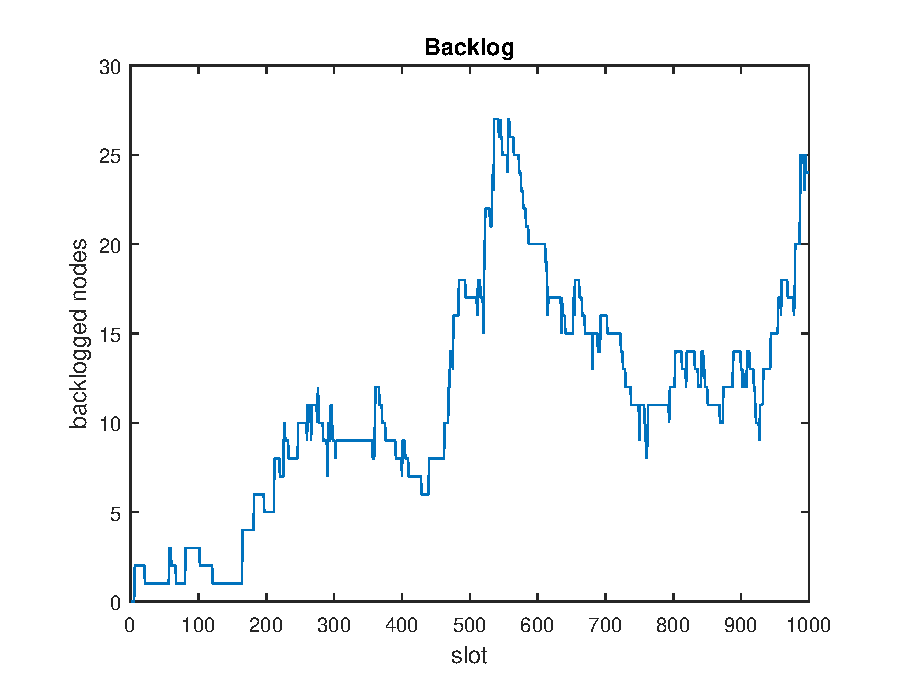
\includegraphics[width=\textwidth]{figures/backlog.eps}
    \caption{Backlog}
    \label{fig:backlog}
  \end{subfigure}%
  \begin{subfigure}{.5\textwidth}
    \includegraphics[width=\textwidth]{figures/arrival-departure-einv.eps}
    \caption{Arrival and departure}
    \label{fig:arrival-departure}
  \end{subfigure}
  \caption{}
\end{figure}

\begin{figure}
  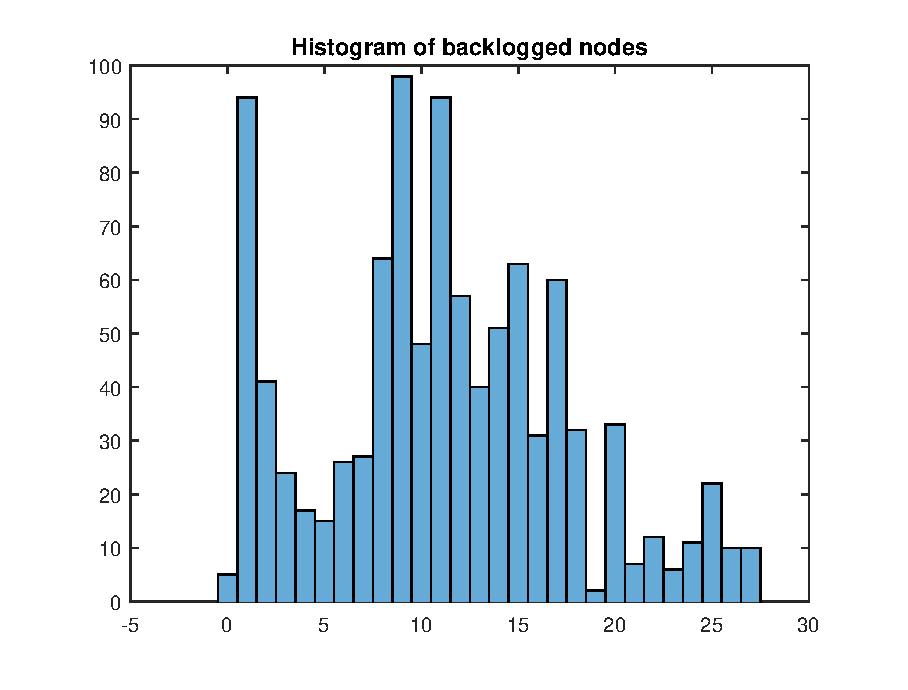
\includegraphics[width=.5\textwidth]{figures/hist-backlog.esp}
\end{figure}
\caption{Histogram of backlog}


\end{document}